% lecture06.tex: Lecture 6: Atmospheres II, Clouds, Weather, & Climate
% Planetary Systems, Kapteyn Institute

\documentclass[aspectratio=169, 11pt]{beamer}

% ── Theme and macros ────────────────────────────────────────
\usepackage{../common/beamerthemeIPS}
% macros.tex: Shared math macros for IPS lecture slides
% Mirrors definitions in book/_config.yml for consistency
% Uses \providecommand to avoid conflicts with unicode-math

% ── Derivatives ─────────────────────────────────────────────
\providecommand{\dv}[2]{\frac{\mathrm{d} #1}{\mathrm{d} #2}}
\providecommand{\dd}{}\renewcommand{\dd}{\mathrm{d}}
\providecommand{\pdv}[2]{\frac{\partial #1}{\partial #2}}

% ── Solar quantities ────────────────────────────────────────
\newcommand{\Msun}{M_{\odot}}
\newcommand{\Rsun}{R_{\odot}}
\newcommand{\Lsun}{L_{\odot}}

% ── Planetary quantities ────────────────────────────────────
\newcommand{\Mearth}{M_{\oplus}}
\newcommand{\Rearth}{R_{\oplus}}
\newcommand{\Mjup}{M_{\mathrm{J}}}
\newcommand{\Rjup}{R_{\mathrm{J}}}

% ── Constants ───────────────────────────────────────────────
\newcommand{\kB}{k_{\mathrm{B}}}

% ── Media links ─────────────────────────────────────────────
% Clickable button that opens the animated or video version of a
% figure, e.g. \mediabutton{https://...gif}{Play animation}
\providecommand{\mediabutton}[2]{\href{#1}{\beamergotobutton{#2}}}

\graphicspath{{figures/}{../common/}{../../book/06_atmospheres_2/figures/}}

% ── Metadata ────────────────────────────────────────────────
\title[Lecture 6: Atmospheres II]{Lecture 6: Atmospheres II\\Clouds, Weather, \& Climate}
\subtitle{Planetary Systems}
\author[L6]{Mara Attia}
\institute{Kapteyn Astronomical Institute\\University of Groningen}
\date{2026}
\titlebgcredit{Jupiter's atmosphere. Credit: NASA/JPL-Caltech/SwRI/MSSS}

% ════════════════════════════════════════════════════════════
\begin{document}

% ── Title slide ─────────────────────────────────────────────
\begin{frame}[plain,noframenumbering]
  \titlepage
\end{frame}

% ── Learning objectives ─────────────────────────────────────
\begin{frame}{Learning objectives}
  By the end of this lecture, you will be able to:
  \vskip8pt
  \begin{itemize}
    \item Derive the Clausius-Clapeyron equation and predict cloud formation
    \item Explain circulation using the Coriolis effect and geostrophic balance
    \item Describe weather phenomena throughout the solar system
    \item Discuss climate evolution and the faint young Sun paradox
    \item Explain the carbonate-silicate cycle as a climate thermostat
  \end{itemize}
\end{frame}

% ── Recap ───────────────────────────────────────────────────
\begin{frame}{Recap: Lecture 5}
  \begin{itemize}
    \item Hydrostatic equilibrium $\dd P = -\rho g\,\dd z$ and scale height $H = \kB T / (\mu\,m_u\,g)$ set atmospheric structure
    \item Radiative equilibrium and greenhouse warming set surface temperatures ($T_s > T_{\mathrm{eq}}$)
    \item Convection drives the adiabatic lapse rate $\Gamma_d = g / c_p$ in the lower atmosphere
  \end{itemize}
  \vskip8pt
  \textbf{Today:} What happens when vapour condenses? How do winds blow? Why has Earth's climate been stable for 4~Gyr?
\end{frame}


% ════════════════════════════════════════════════════════════
\sectionimage{titan_clouds}{Methane clouds over Titan, Cassini ISS. Credit: NASA/JPL-Caltech/SSI}
\section{Cloud formation}
% ════════════════════════════════════════════════════════════

% ── Saturation ───────────────────────────────────────────────
\begin{frame}{Saturation and condensation}
  \begin{itemize}
    \item Every vapour has a \textbf{saturation vapour pressure} $P_{\mathrm{sat}}(T)$
    \item When actual vapour pressure exceeds $P_{\mathrm{sat}}$: air is \textbf{supersaturated}
    \item $P_{\mathrm{sat}}(T)$ increases roughly exponentially with temperature
    \item \textbf{Relative humidity:}
    $$\mathrm{RH} = \frac{P_{\mathrm{vapour}}}{P_{\mathrm{sat}}(T)} \times 100\%$$
    \item $\mathrm{RH} = 100\%$: saturated; $\mathrm{RH} > 100\%$: condensation can occur
    \item Rising air cools $\rightarrow$ $P_{\mathrm{sat}}$ drops $\rightarrow$ reaches saturation $\rightarrow$ clouds
  \end{itemize}
\end{frame}

% ── Saturation curves hero ──────────────────────────────────
\begin{frame}
  \centering
  \makebox[\linewidth][c]{
\includegraphics[width=0.95\paperwidth, height=0.72\paperheight, keepaspectratio]{psat_curves}}\\
  {\footnotesize Saturation vapour pressure for the five main condensables. A single equation, evaluated per species, predicts every cloud deck in the solar system. Course figure.}
\end{frame}

% ── Nucleation ──────────────────────────────────────────────
\begin{frame}{Nucleation: how droplets form}
  Even in supersaturated air, condensation needs a \textbf{seed}.
  \vskip6pt
  \begin{description}\setlength\itemsep{4pt}
    \item[Homogeneous nucleation:] Droplets from vapour alone; requires extreme supersaturation ($\mathrm{RH} \gg 100\%$), very rare
    \item[Heterogeneous nucleation:] Condensation onto pre-existing nuclei (dust, sea salt, soot); activates at only $\sim$0.04--0.4\% supersaturation
  \end{description}
  \vskip6pt
  \begin{itemize}
    \item Earth: oceanic/biogenic nuclei; Mars: dust; Giant planets: photochemical hazes
  \end{itemize}
\end{frame}

% ── Köhler curves hero ──────────────────────────────────────
\begin{frame}
  \centering
  \makebox[\linewidth][c]{\includegraphics[width=0.95\paperwidth, height=0.72\paperheight, keepaspectratio]{kohler_curves}}\\
  {\footnotesize K\"ohler curves: equilibrium supersaturation of solution droplets. Real clouds nucleate heterogeneously, with aerosols lowering the barrier by two orders of magnitude. Course figure.}
\end{frame}

% ── Lifting condensation level ──────────────────────────────
\begin{frame}{The lifting condensation level (LCL)}
  \begin{columns}[c]
    \column{\recapfigcol}
    \ipsrecapfig{cumulonimbus_anvil}
    \source{Eulenj\"ager, CC BY-SA 3.0}

    \column{\recaptextcol}
    \footnotesize
    Rising air cools dry adiabatically ($\Gamma_d = g/c_p$) until $P_{\mathrm{vapour}} = P_{\mathrm{sat}}(T)$, i.e.\ until it reaches its \textbf{dew point} $T_d$.
    \vskip4pt
    \keyresult{The \textbf{lifting condensation level} (LCL) marks the \textbf{cloud base}.}
    \vskip4pt
    \begin{itemize}\setlength\itemsep{2pt}
      \item Above the LCL, latent heat release reduces cooling to the moist adiabatic lapse rate ($\sim$5~K\,km$^{-1}$ vs.\ $\sim$9.8~K\,km$^{-1}$ dry)
      \item Latent heat fuels buoyancy, powering deep convective storms up to the tropopause
    \end{itemize}
  \end{columns}
\end{frame}

% ── Cloud types across solar system ─────────────────────────
\begin{frame}{Cloud types of the solar system}
  What condenses depends on temperature and composition:
  \vskip6pt
  \centering
  \small
  \begin{tabular}{l l l}
    \toprule
    \textbf{Body} & \textbf{Cloud species} & \textbf{Cloud base altitude} \\
    \midrule
    Earth    & $\mathrm{H_2O}$                          & $\sim$1--2~km \\
    Venus    & $\mathrm{H_2SO_4}$                       & $\sim$48~km \\
    Mars     & $\mathrm{CO_2}$ ice, $\mathrm{H_2O}$ ice & 10--100~km \\
    Titan    & $\mathrm{CH_4}$, $\mathrm{C_2H_6}$       & $\sim$8--30~km \\
    Jupiter  & $\mathrm{NH_3}$, $\mathrm{NH_4SH}$, $\mathrm{H_2O}$ & layered, 0.5--7~bar \\
    \bottomrule
  \end{tabular}
  \vskip8pt
  \flushleft
  The \textbf{Clausius-Clapeyron equation} governs every cloud deck.
\end{frame}

\begin{frame}
  \centering
  \makebox[\linewidth][c]{\includegraphics[width=0.95\paperwidth, height=0.66\paperheight, keepaspectratio]{cloud_species_map}}\\
  {\footnotesize Which species condenses where: H$_2$O clouds with a base at 1 to 2 km on Earth, H$_2$SO$_4$ droplets at 48 to 70 km on Venus, CO$_2$ and H$_2$O ice clouds at high altitude on Mars, CH$_4$ and C$_2$H$_6$ clouds near Titan's surface, and the NH$_3$, NH$_4$SH and H$_2$O decks at successively deeper levels on Jupiter and Saturn. The same Clausius-Clapeyron physics governs every case; only the species and its condensation temperature differ. Course schematic.}
\end{frame}


% ════════════════════════════════════════════════════════════
\sectionimage{venus_uv_clouds}{Venus in UV. Credit: NASA/JPL-Caltech}
\section{Blackboard derivation: the Clausius-Clapeyron equation}
% ════════════════════════════════════════════════════════════

% ── Setup ────────────────────────────────────────────────────
\begin{frame}{Deriving the Clausius-Clapeyron equation}
  \textbf{Goal:} Derive the exponential dependence of saturation vapour pressure on temperature from thermodynamic phase equilibrium.
  \vskip10pt
  \textbf{Setup: phase equilibrium.}
  \vskip6pt
  Along the coexistence curve, liquid and vapour are in equilibrium:
  $$g_\ell(T, P) = g_v(T, P)$$
  where $g$ is the specific Gibbs free energy.
  \vskip6pt
  Moving along the coexistence curve by $(\dd T, \dd P)$:
  $$\dd g_\ell = \dd g_v$$
  \vskip8pt
  \textit{To the board.}
\end{frame}

% ── Result ──────────────────────────────────────────────────
\begin{frame}{The Clausius-Clapeyron equation}
  \keyresult{$$\boxed{P_{\mathrm{sat}}(T) = P_{\mathrm{ref}} \exp\!\left[-\frac{L_v}{R_v}\left(\frac{1}{T} - \frac{1}{T_{\mathrm{ref}}}\right)\right]}$$}
  \source{Derivation follows Catling (2017), \textit{Atmospheric Evolution on Inhabited and Lifeless Worlds}, Ch.~1}
  \vskip8pt
  \begin{itemize}
    \item $P_{\mathrm{sat}}$ depends \textbf{exponentially} on temperature
    \item The sensitivity is controlled by $L_v/R_v$ (units of K)
    \item Large $L_v/R_v$ $\rightarrow$ very sensitive to temperature changes
    \item This equation applies to \textbf{any} vapour $\leftrightarrow$ condensed phase transition
  \end{itemize}
\end{frame}

\begin{frame}
  \centering
  \makebox[\linewidth][c]{\includegraphics[width=0.95\paperwidth, height=0.72\paperheight, keepaspectratio]{water_phase_diagram}}\\
  {\footnotesize Phase diagram of water in $P$-$T$ space. The liquid-vapour coexistence curve integrates the Clausius-Clapeyron relation from the triple point to the critical point; the solid-vapour curve governs sublimation. Course figure.}
\end{frame}

% ── Worked example: water ──────────────────────────────────
\begin{frame}{Worked example: water on Earth}
  For water vapour:
  \vskip4pt
  \centering
  \begin{tabular}{l r}
    \toprule
    $L_v$ & $2.50 \times 10^6$~J\,kg$^{-1}$ \\
    $M$ & 0.018~kg\,mol$^{-1}$ \\
    $R_v = R^*/M$ & 462~J\,kg$^{-1}$\,K$^{-1}$ \\
    $T_{\mathrm{ref}}$ (triple point) & 273~K \\
    $P_{\mathrm{ref}}$ (triple point) & 611~Pa \\
    \midrule
    $L_v/R_v$ & $\approx 5400$~K \\
    \bottomrule
  \end{tabular}
  \vskip8pt
  \flushleft
  At $T = 293$~K (20\textdegree{}C):
  $$P_{\mathrm{sat}} = 611 \exp\!\left[-5400\left(\frac{1}{293} - \frac{1}{273}\right)\right] = 611 \times 3.86 \approx 2360 \text{~Pa}$$
  Measured value: 2300~Pa; excellent agreement.
\end{frame}

% ── Condensing species table ────────────────────────────────
\begin{frame}{Condensing species in the solar system}
  \centering
  \footnotesize
  \begin{tabular}{l c c c c l}
    \toprule
    \textbf{Species} & $L_v$ (kJ\,kg$^{-1}$) & $R_v$ (J\,kg$^{-1}$\,K$^{-1}$) & $L_v/R_v$ (K) & $T_{\mathrm{cond}}$ (K) & \textbf{Where} \\
    \midrule
    $\mathrm{H_2O}$      & 2500 & 462 & 5400 & 200--280 & Earth, Mars \\
    $\mathrm{H_2SO_4}$   & 540  & 85  & 6400 & 230--360 & Venus \\
    $\mathrm{NH_3}$      & 1370 & 488 & 2800 & 130--150 & Jupiter, Saturn \\
    $\mathrm{CH_4}$      & 510  & 519 & 980  & 80--90   & Titan, Uranus, Neptune \\
    $\mathrm{CO_2}$      & 571  & 189 & 3020 & 100--150 & Mars \\
    \bottomrule
  \end{tabular}
  \vskip6pt
  \keyresult{Steep $L_v/R_v$ curves sharpen cloud bases (Venus); flat curves broaden decks (Titan).}
\end{frame}


% ════════════════════════════════════════════════════════════
\sectionimage{mars_water_ice_clouds}{Water-ice clouds over Mars, Mars Odyssey THEMIS (2025). Credit: NASA/JPL-Caltech/ASU}
\section{Clouds of the solar system}
% ════════════════════════════════════════════════════════════

% ── Venus clouds ────────────────────────────────────────────
\begin{frame}{Venus: sulfuric acid clouds}
  \begin{columns}[c]
    \column{\recapfigcolnarrow}
    \centering
    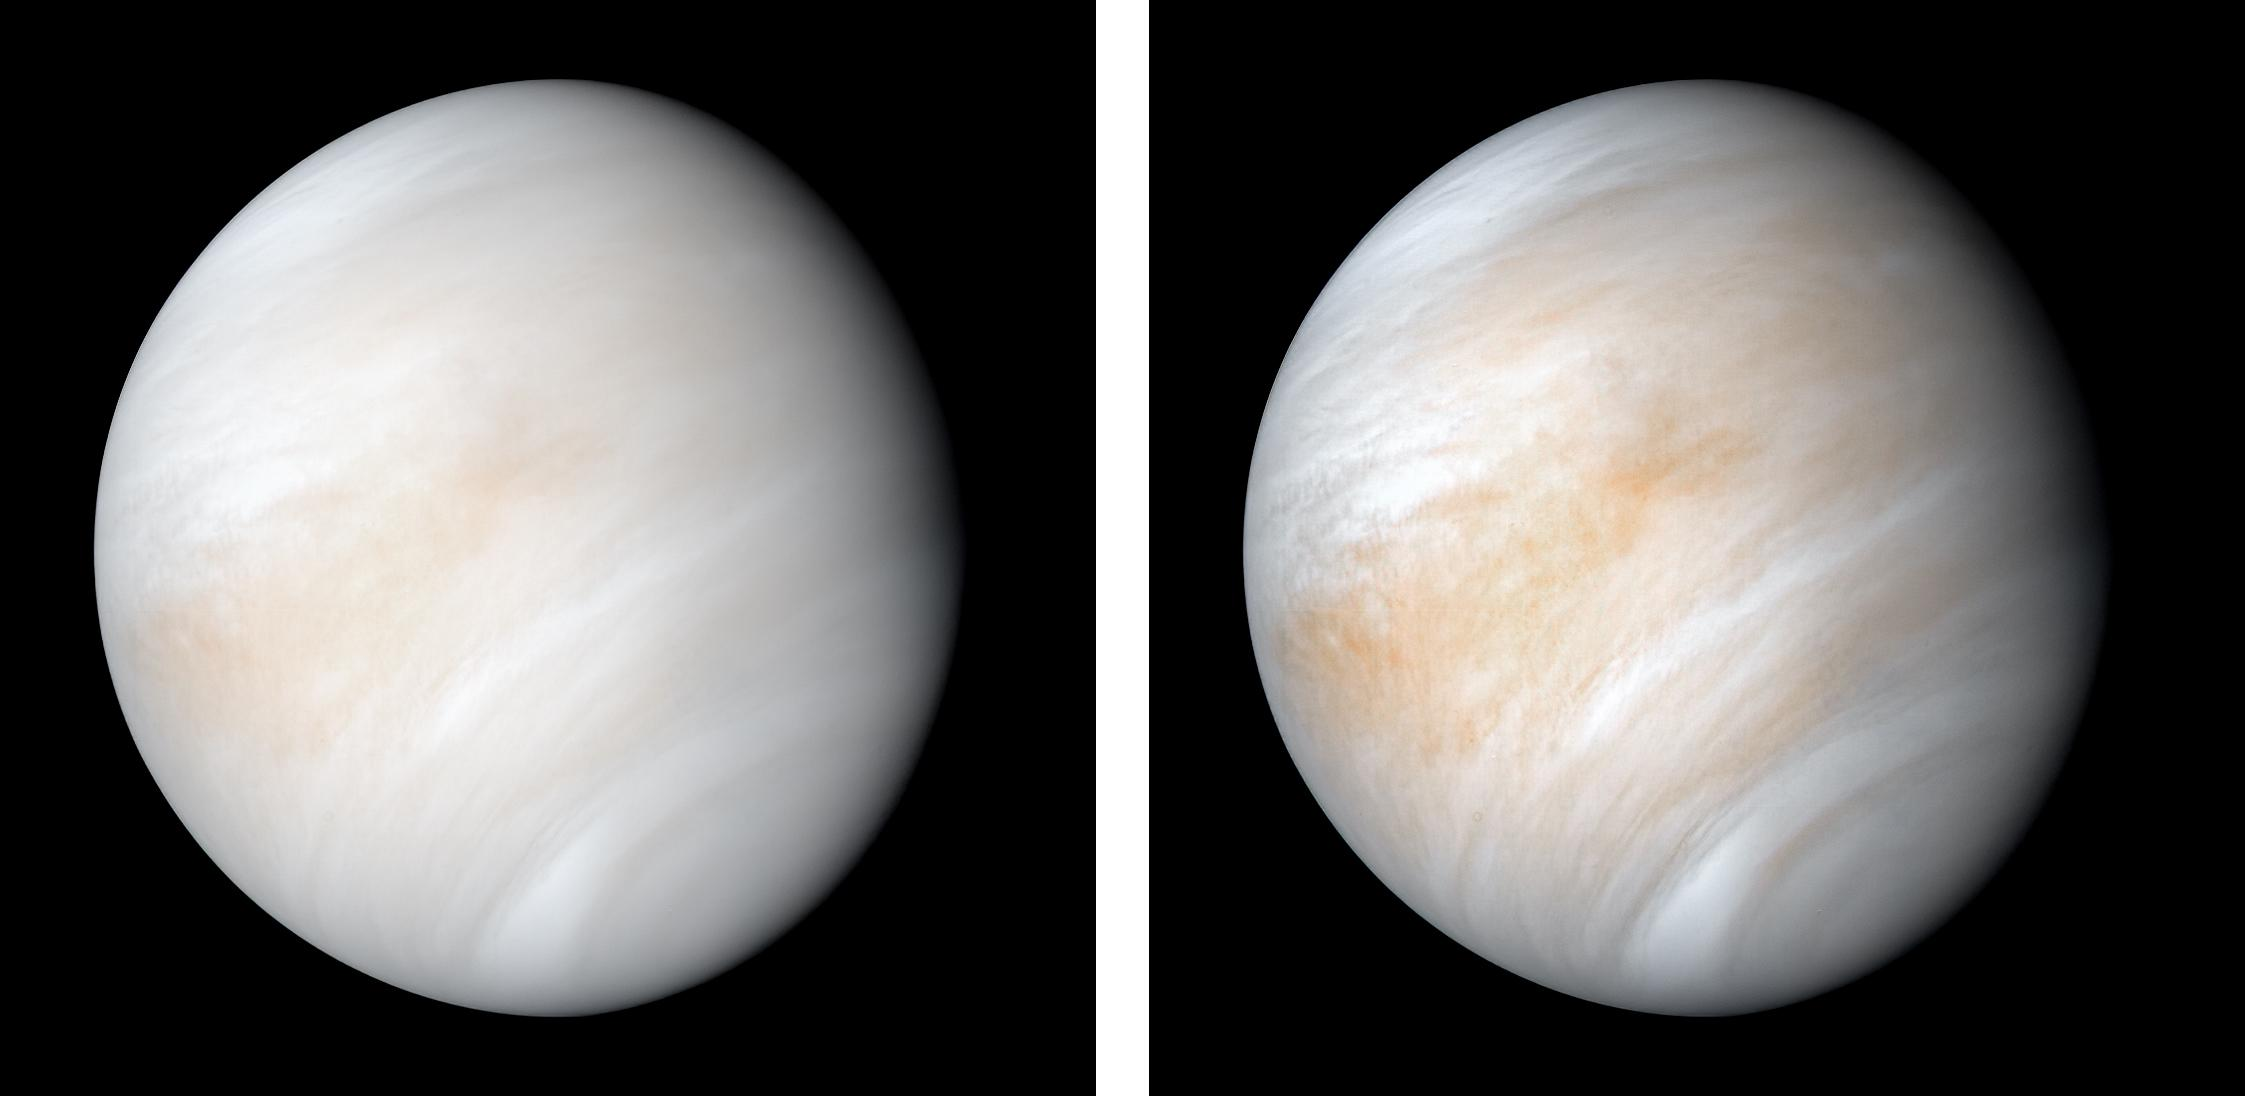
\includegraphics[width=\linewidth,height=0.62\textheight,keepaspectratio]{venus_uv_clouds}
    \source{NASA/JPL-Caltech (1974)}

    \column{\recaptextcolwide}
    \footnotesize
    \begin{itemize}\setlength\itemsep{2pt}
      \item Concentrated $\mathrm{H_2SO_4}$ clouds span 48--70~km altitude
      \item Photochemistry from outgassed $\mathrm{SO_2}$ and photolytic O:
      $$\mathrm{SO_2} + \mathrm{O} \rightarrow \mathrm{SO_3}, \;\, \mathrm{SO_3} + \mathrm{H_2O} \rightarrow \mathrm{H_2SO_4}$$
      \item Unidentified UV absorber creates upper-cloud tracking features
      \item Sub-cloud haze extends down to $\sim$31~km
    \end{itemize}
  \end{columns}
\end{frame}

% ── Venus T-z profile hero ──────────────────────────────────
\begin{frame}
  \centering
  \makebox[\linewidth][c]{\includegraphics[width=0.95\paperwidth, height=0.72\paperheight, keepaspectratio]{venus_tz_profile}}\\
  {\footnotesize Venus thermal structure, VIRA / Venus Express VeRa. Concentrated $\mathrm{H_2SO_4}$ clouds form a 22~km deck at 48--70~km altitude where Clausius-Clapeyron allows them. Course figure.}
\end{frame}

% ── Mars clouds ─────────────────────────────────────────────
\begin{frame}{Mars: dust and ice clouds}
  \centering
  \makebox[\linewidth][c]{\includegraphics[width=0.75\linewidth]{mars_water_ice_clouds}}
  {\tiny\color{ipsText!60} Water-ice clouds over Tharsis limb. Credit: NASA/JPL-Caltech/ASU (Mars Odyssey THEMIS, 2 May 2025)}
  \vskip2pt
  \raggedright\footnotesize
  \begin{columns}[T]
    \column{0.52\textwidth}
    \begin{itemize}\setlength\itemsep{1pt}
      \item \textbf{$\mathrm{CO_2}$ ice:} mesospheric, 50--100~km, where $T$ falls below the local $\mathrm{CO_2}$ frost point (148~K at the 6~mbar surface, lower aloft)
      \item \textbf{$\mathrm{H_2O}$ ice:} 10--30~km over Tharsis volcanoes
    \end{itemize}
    \column{0.46\textwidth}
    \begin{itemize}\setlength\itemsep{1pt}
      \item Mineral dust acts as condensation nuclei
      \item Radiative heating drives positive dust feedback
    \end{itemize}
  \end{columns}
\end{frame}

% ── Titan methane cycle ─────────────────────────────────────
\begin{frame}{Titan's methane cycle: an Earthlike analogue}
  \begin{columns}[c]
    \column{\recapfigcolnarrow}
    \centering
    \includegraphics[width=\linewidth,height=0.62\textheight,keepaspectratio]{titan_lakes}
    \source{NASA/JPL-Caltech/ASI/USGS (Cassini)}

    \column{\recaptextcolwide}
    \footnotesize
    Active hydrological cycle with $\mathrm{CH_4}$ near its triple point:
    \vskip4pt
    \begin{itemize}\setlength\itemsep{2pt}
      \item Surface at 94~K and 1.5~bar supports liquid methane seas
      \item \textbf{Kraken Mare:} $\sim$400{,}000~km$^2$, locally $>$100~m deep
      \item Methane rain carves river channels and fills polar lakes
      \item Driven by slow 30-year seasonal solar cycling
    \end{itemize}
  \end{columns}
\end{frame}

% ── Titan clouds hero ───────────────────────────────────────
\begin{frame}
  \centering
  \makebox[\linewidth][c]{\includegraphics[width=0.95\paperwidth, height=0.72\paperheight, keepaspectratio]{titan_clouds}}\\
  {\footnotesize Methane clouds at Titan's mid-southern latitudes, Cassini ISS. Methane rain at 94~K drives the only active hydrological cycle beyond Earth with polar convective storms. Credit: NASA/JPL-Caltech/SSI.}
\end{frame}

% ── Giant planet cloud layers ────────────────────────────────
\begin{frame}{Giant planets: layered cloud structure}
  \begin{columns}[c]
    \column{\recapfigcolnarrow}
    \centering
    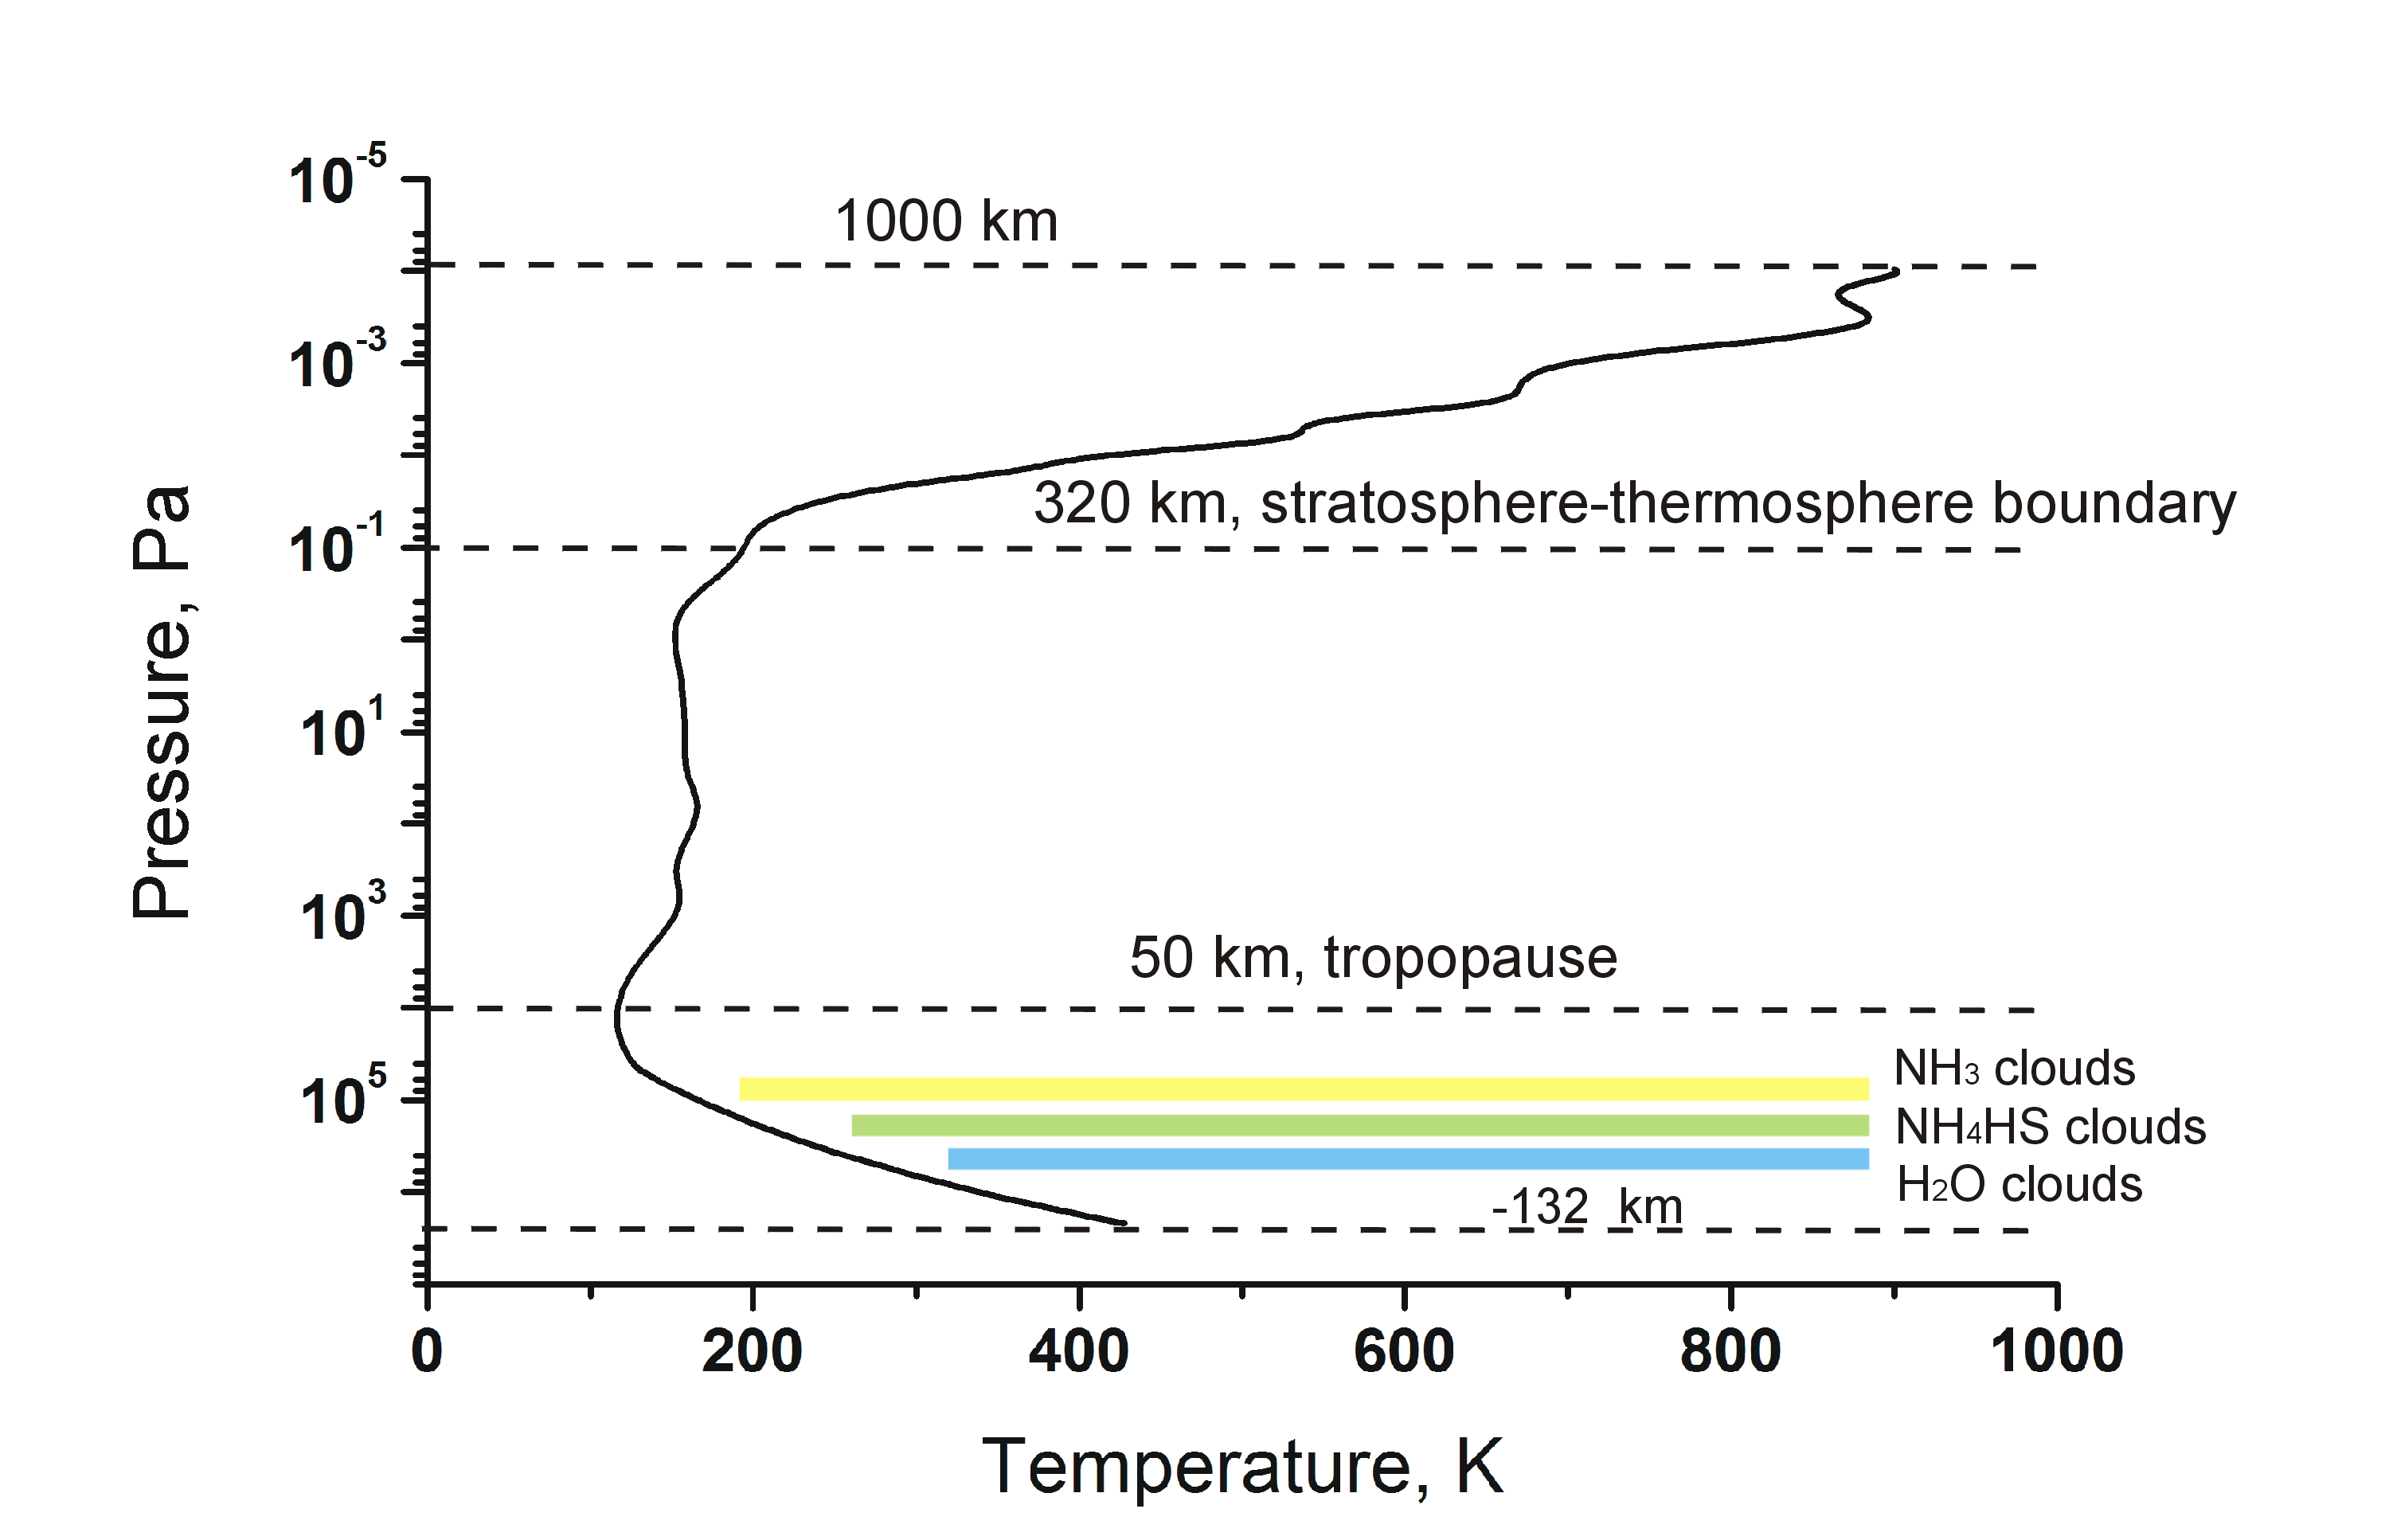
\includegraphics[width=\linewidth,height=0.62\textheight,keepaspectratio]{jupiter_cloud_layers}
    \source{Wikimedia, CC BY-SA 3.0}

    \column{\recaptextcolwide}
    \footnotesize
    Vertically layered, predicted by Clausius-Clapeyron:
    \vskip4pt
    \begin{enumerate}\setlength\itemsep{2pt}
      \item \textbf{$\mathrm{NH_3}$ ice} (top): 130--150~K, 0.5--1~bar
      \item \textbf{$\mathrm{NH_4SH}$}: 200--240~K, 2--3~bar ($\mathrm{NH_3} + \mathrm{H_2S}$)
      \item \textbf{$\mathrm{H_2O}$ ice/liquid} (deep): 270--300~K, 5--7~bar
    \end{enumerate}
    \vskip4pt
    Latent heat release from deep water clouds fuels moist convection.
  \end{columns}
\end{frame}


% ════════════════════════════════════════════════════════════
\sectionimage{earth_jet_stream}{Jet-stream cirrus from orbit. Credit: NASA/JSC}
\section{Atmospheric dynamics}
% ════════════════════════════════════════════════════════════

% ── Hadley cell ─────────────────────────────────────────────
\begin{frame}{The Hadley cell}
  \begin{columns}[c]
    \column{\recapfigcolnarrow}
    \centering
    \includegraphics[width=\linewidth,height=0.62\textheight,keepaspectratio]{hadley_observed}
    \source{Course figure}

    \column{\recaptextcolwide}
    \footnotesize
    \begin{enumerate}\setlength\itemsep{2pt}
      \item Solar heating at the equator drives buoyant rising air
      \item Air flows poleward aloft, cooling radiatively
      \item Sinking air at $\sim$30\textdegree{} latitude creates subtropical desert belts
      \item Equatorward surface return flow forms the trade winds
    \end{enumerate}
    \vskip4pt
    \keyresult{The primary tropical heat transport loop from equator to mid-latitudes.}
  \end{columns}
\end{frame}

% ── Coriolis effect ─────────────────────────────────────────
\begin{frame}{The Coriolis effect}
  On a rotating planet, moving air is deflected right in the Northern Hemisphere, left in the Southern.
  \vskip6pt
  The \textbf{Coriolis parameter}:
  $$f = 2\Omega \sin\phi$$
  \vskip4pt
  \begin{itemize}\setlength\itemsep{2pt}
    \item Earth: $\Omega = 7.29 \times 10^{-5}$~rad\,s$^{-1}$
    \item Mid-latitudes ($\phi = 45$\textdegree{}): $f \approx 1.03 \times 10^{-4}$~s$^{-1}$
    \item Equator ($\phi = 0$\textdegree{}): $f = 0$, so no Coriolis deflection
  \end{itemize}
  \vskip4pt
  \keyresult{Explains why winds circulate around pressure centres instead of blowing directly from high to low.}
\end{frame}

% ── Coriolis deflection hero ────────────────────────────────
\begin{frame}
  \centering
  \makebox[\linewidth][c]{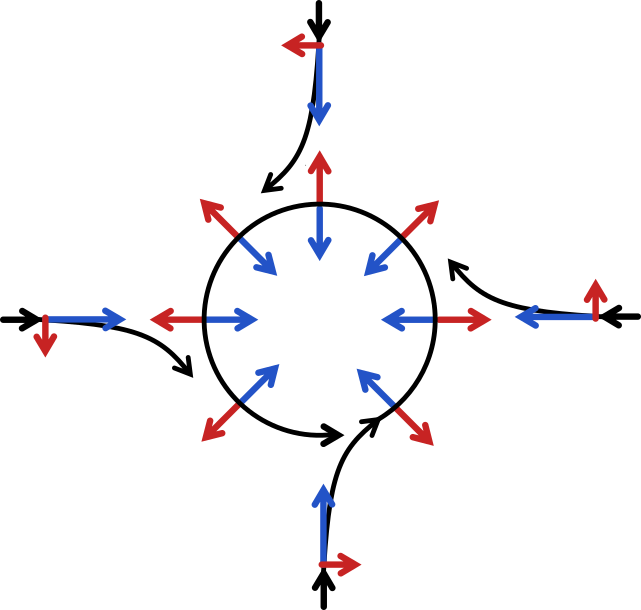
\includegraphics[width=0.95\paperwidth, height=0.72\paperheight, keepaspectratio]{coriolis_effect}}\\
  {\footnotesize Coriolis deflection of a polar launch, viewed from above the North Pole. The deflection is an apparent force caused by the planet rotating beneath a straight path. Course figure.}
\end{frame}

% ── Rossby number ───────────────────────────────────────────
\begin{frame}{The Rossby number}
  Does planetary rotation dominate a given atmospheric flow?
  \vskip6pt
  $$\mathrm{Ro} = \frac{U}{fL}$$
  \vskip4pt
  \begin{description}\setlength\itemsep{3pt}
    \item[$\mathrm{Ro} \ll 1$:] Rotation dominates: large-scale circulation, jet streams (Earth: $U \sim 10$~m\,s$^{-1}$, $L \sim 1000$~km $\rightarrow \mathrm{Ro} \sim 0.1$)
    \item[$\mathrm{Ro} \gg 1$:] Rotation unimportant: small-scale convective plumes, tornadoes
  \end{description}
  \vskip4pt
  \keyresult{The Rossby number sets the dynamic regime and the number of circulation cells.}
\end{frame}

\begin{frame}
  \centering
  \makebox[\linewidth][c]{\includegraphics[width=0.95\paperwidth, height=0.66\paperheight, keepaspectratio]{rossby_regimes}}\\
  {\footnotesize Flow regimes sorted by $\mathrm{Ro} = U/(fL)$ for mid-latitude Earth ($f = 10^{-4}$ s$^{-1}$): large-scale circulation ($U \sim 10$ m\,s$^{-1}$, $L \sim 1000$ km, $\mathrm{Ro} \sim 0.1$) lies where rotation dominates; a dust devil (about 10 m, 10 m\,s$^{-1}$) and a tornado (about 100 m, 50 m\,s$^{-1}$) lie far inside the region where pressure gradients and friction govern the flow. Course figure.}
\end{frame}

% ── Circulation cells vs rotation ──────────────────
\begin{frame}{Circulation cells and rotation rate}
  \begin{columns}[c]
    \column{\recapfigcolnarrow}
    \ipsrecapfig{hadley_cells}
    \source{Wikimedia Commons, public domain}

    \column{\recaptextcolwide}
    \footnotesize
    Planetary rotation rate governs the number of circulation cells:
    \vskip4pt
    \begin{itemize}\setlength\itemsep{2pt}
      \item \textbf{Slow rotators} (Venus, Titan): single equator-to-pole Hadley cell per hemisphere ($\mathrm{Ro} \gg 1$)
      \item \textbf{Moderate rotators} (Earth): three cells (Hadley, Ferrel, polar)
      \item \textbf{Fast rotators} (Jupiter, Saturn): multiple cells produce banded jets
    \end{itemize}
  \end{columns}
\end{frame}


% ── Break ───────────────────────────────────────────────────
\breakslide


% ════════════════════════════════════════════════════════════
\sectionimage{saturn_hexagon}{Saturn's hexagonal jet stream, Cassini. Credit: NASA/JPL-Caltech/SSI}
\section{Geostrophic balance \& jet streams}
% ════════════════════════════════════════════════════════════

% ── Geostrophic balance ─────────────────────────────────────
\begin{frame}{Geostrophic balance}
  \begin{columns}[c]
    \column{\recapfigcolnarrow}
    \ipsrecapfig{geostrophic_balance}

    \column{\recaptextcolwide}
    \footnotesize
    At large scales ($\mathrm{Ro} \ll 1$), Coriolis force balances pressure gradient:
    $$f\,\hat{k} \times \mathbf{v}_g = -\frac{1}{\rho}\nabla P$$
    $$u_g = -\frac{1}{f\rho}\pdv{P}{y}, \qquad v_g = \frac{1}{f\rho}\pdv{P}{x}$$
    \vskip2pt
    \keyresult{Geostrophic winds blow \textbf{parallel to isobars}, rotating cyclonically around lows and anticyclonically around highs.}
  \end{columns}
\end{frame}

% ── Jet streams and the thermal wind ─────────────────────────
\begin{frame}{Jet streams and the thermal wind}
  \begin{columns}[c]
    \column{\recapfigcol}
    \ipsrecapfig{earth_jet_stream}
    \source{NASA JSC, public domain}

    \column{\recaptextcol}
    \footnotesize
    Horizontal temperature gradients drive vertical wind shear through the thermal wind relation:
    $$\pdv{\mathbf{v}_g}{z} \propto \hat{k} \times \nabla T$$
    \vskip4pt
    \begin{itemize}\setlength\itemsep{2pt}
      \item Steep equator-to-pole $\nabla T$ drives fast winds aloft ($\sim$30--70~m\,s$^{-1}$ on Earth)
      \item Earth hosts subtropical ($\sim$30\textdegree{}) and polar ($\sim$60\textdegree{}) jet streams
      \item Upper-tropospheric jets steer mid-latitude weather systems across the globe
    \end{itemize}
  \end{columns}
\end{frame}

% ── Jupiter zonal winds hero ────────────────────────────────
\begin{frame}
  \centering
  \makebox[\linewidth][c]{\includegraphics[width=0.95\paperwidth, height=0.72\paperheight, keepaspectratio]{jupiter_zonal_winds}}\\
  {\footnotesize Jupiter's cloud-top zonal winds, schematic after Garc\'ia Melendo \& S\'anchez-Lavega (2001). Alternating prograde and retrograde jets reach peak speeds of $\sim$180~m\,s$^{-1}$ and extend thousands of kilometres deep. Course figure.}
\end{frame}

% ── Giant planet banding ────────────────────────────────────
\begin{frame}{Giant planet banding}
  \begin{columns}[c]
    \column{\recapfigcol}
    \ipsrecapfig{jupiter_global_map}
    \source{NASA/ESA/STScI (HST OPAL)}

    \column{\recaptextcol}
    \footnotesize
    Planetary rotation organises giant-planet atmospheres into alternating bright zones and dark belts:
    \vskip4pt
    \begin{itemize}\setlength\itemsep{2pt}
      \item \textbf{Zones (light):} anticyclonic upwelling, cool ammonia ice cloud tops
      \item \textbf{Belts (dark):} cyclonic downwelling exposing warmer lower layers
      \item Zonal jets flank band boundaries (Jupiter $\sim$180~m\,s$^{-1}$, Saturn $\sim$400~m\,s$^{-1}$); decay depth $\sim$1800~km
    \end{itemize}
  \end{columns}
\end{frame}


% ════════════════════════════════════════════════════════════
\sectionimage{jupiter_great_red_spot}{Jupiter's Great Red Spot. Credit: NASA/JPL-Caltech/SwRI/MSSS}
\section{Weather \& storms in the solar system}
% ════════════════════════════════════════════════════════════

% ── Mars dust storms ────────────────────────────────────────
\begin{frame}{Mars: dust storms}
  \begin{columns}[c]
    \column{\recapfigcolnarrow}
    \centering
    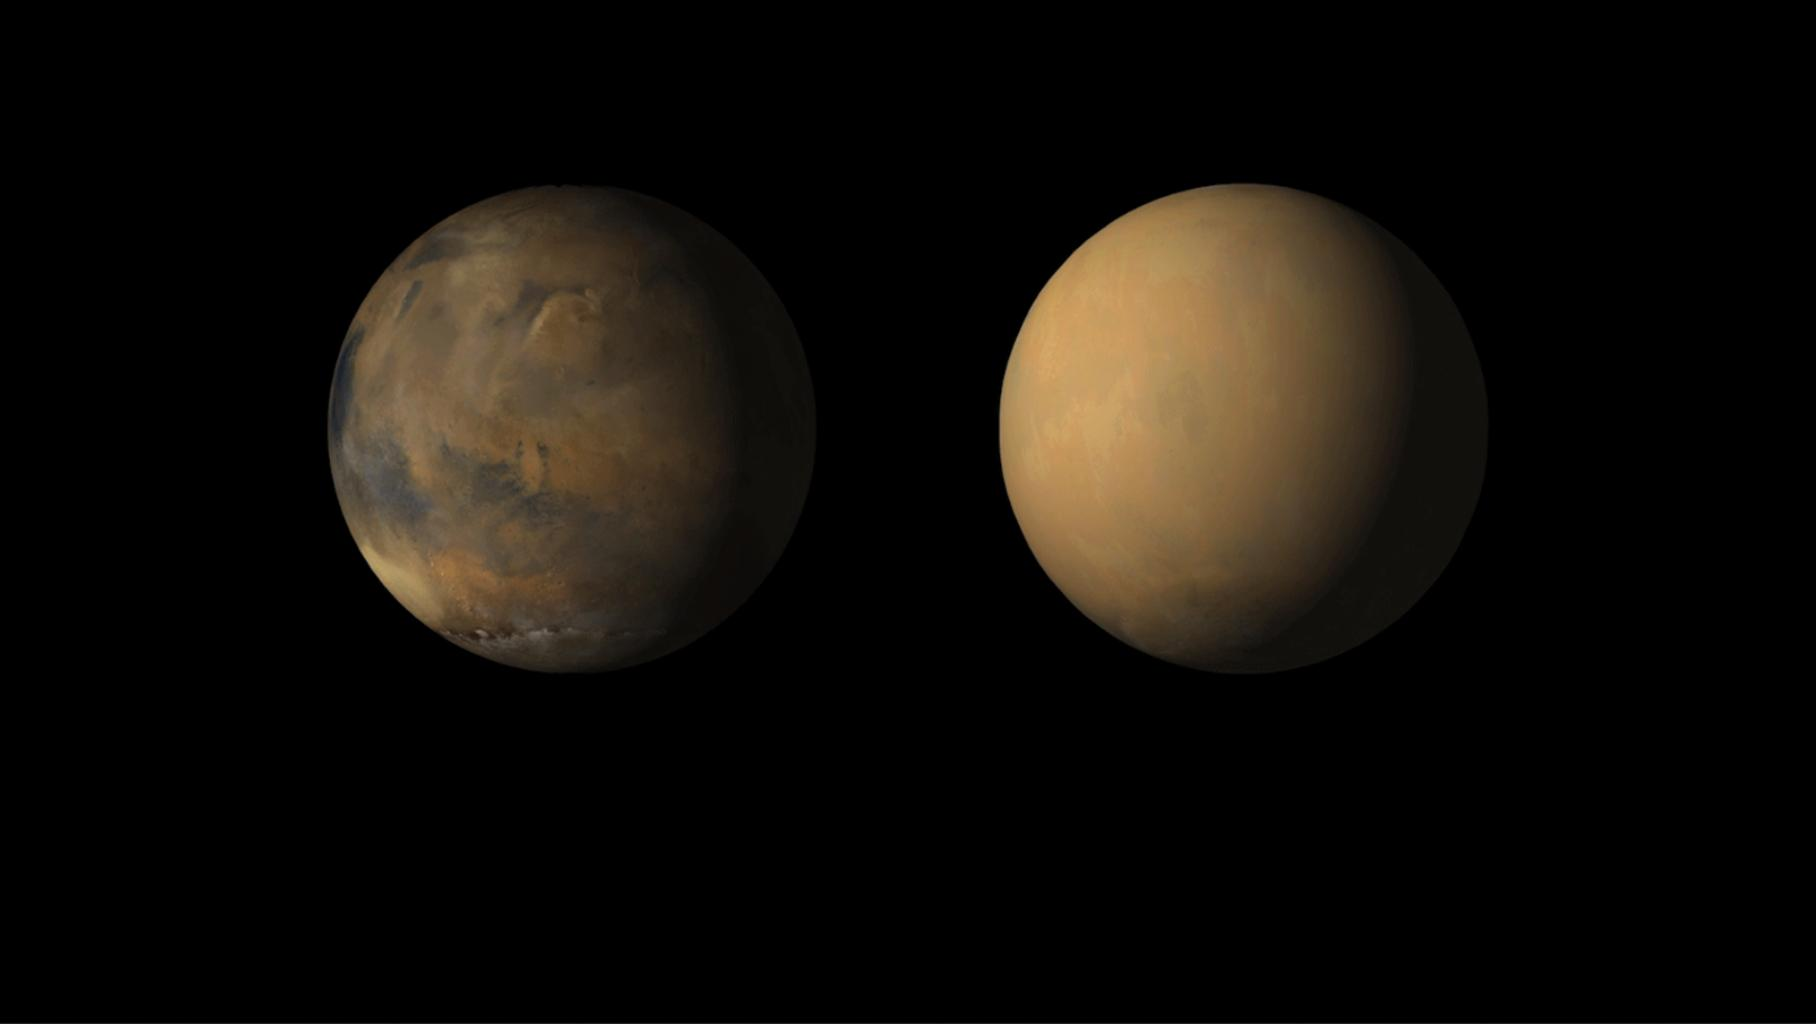
\includegraphics[width=\linewidth,height=0.62\textheight,keepaspectratio]{mars_dust_storm}
    \source{NASA/JPL-Caltech/MSSS}

    \column{\recaptextcolwide}
    \footnotesize
    \begin{itemize}\setlength\itemsep{2pt}
      \item Dust lofted to 10--30~km can grow into global dust storms
      \item \textbf{Positive feedback loop:} dust absorbs sunlight $\rightarrow$ heats air $\rightarrow$ strengthens winds $\rightarrow$ lofts more dust
      \item Seasonal $\mathrm{CO_2}$ condensation freezes 25--30\% of the atmosphere onto polar caps, swinging the surface pressure between $\sim$5 and 7~mbar
    \end{itemize}
  \end{columns}
\end{frame}

% ── Venus winds hero ────────────────────────────────────────
\begin{frame}
  \centering
  \makebox[\linewidth][c]{\includegraphics[width=0.95\paperwidth, height=0.76\paperheight, keepaspectratio]{sanchezlavega2008_venus_winds}}\\
  {\footnotesize Venus cloud-level winds from VIRTIS on Venus Express: zonal (A) and meridional (B) speed against latitude. Cloud-top zonal winds reach $\sim$105~m\,s$^{-1}$, demonstrating that the entire cloud deck super-rotates 60 times faster than the surface. S\'anchez-Lavega et al.\ (2008).}
\end{frame}

% ── Venus super-rotation: thermal tides ────────────
\begin{frame}{Venus super-rotation: thermal tides}
  \begin{columns}[c]
    \column{\recapfigcol}
    \ipsrecapfig{venus_uv_clouds}
    \source{NASA/JPL-Caltech (Mariner 10)}

    \column{\recaptextcol}
    \footnotesize
    Cloud-top winds circle Venus in $\sim$4 days ($\sim$100~m\,s$^{-1}$), 60 times faster than the surface.
    \vskip4pt
    \begin{itemize}\setlength\itemsep{2pt}
      \item \textbf{Puzzle:} sustaining super-rotation requires transporting momentum upward and equatorward
      \item \textbf{Thermal tides:} solar heating generates waves that pump momentum upward
      \item \textbf{Planetary waves:} large-scale waves carry momentum toward the equator
    \end{itemize}
    \vskip4pt
    \sourcenote{S\'{a}nchez-Lavega et al.\ (2017)}
  \end{columns}
\end{frame}

% ── Jupiter GRS ─────────────────────────────────────────────
\begin{frame}{Jupiter: the Great Red Spot}
  \begin{columns}[c]
    \column{\recapfigcolnarrow}
    \centering
    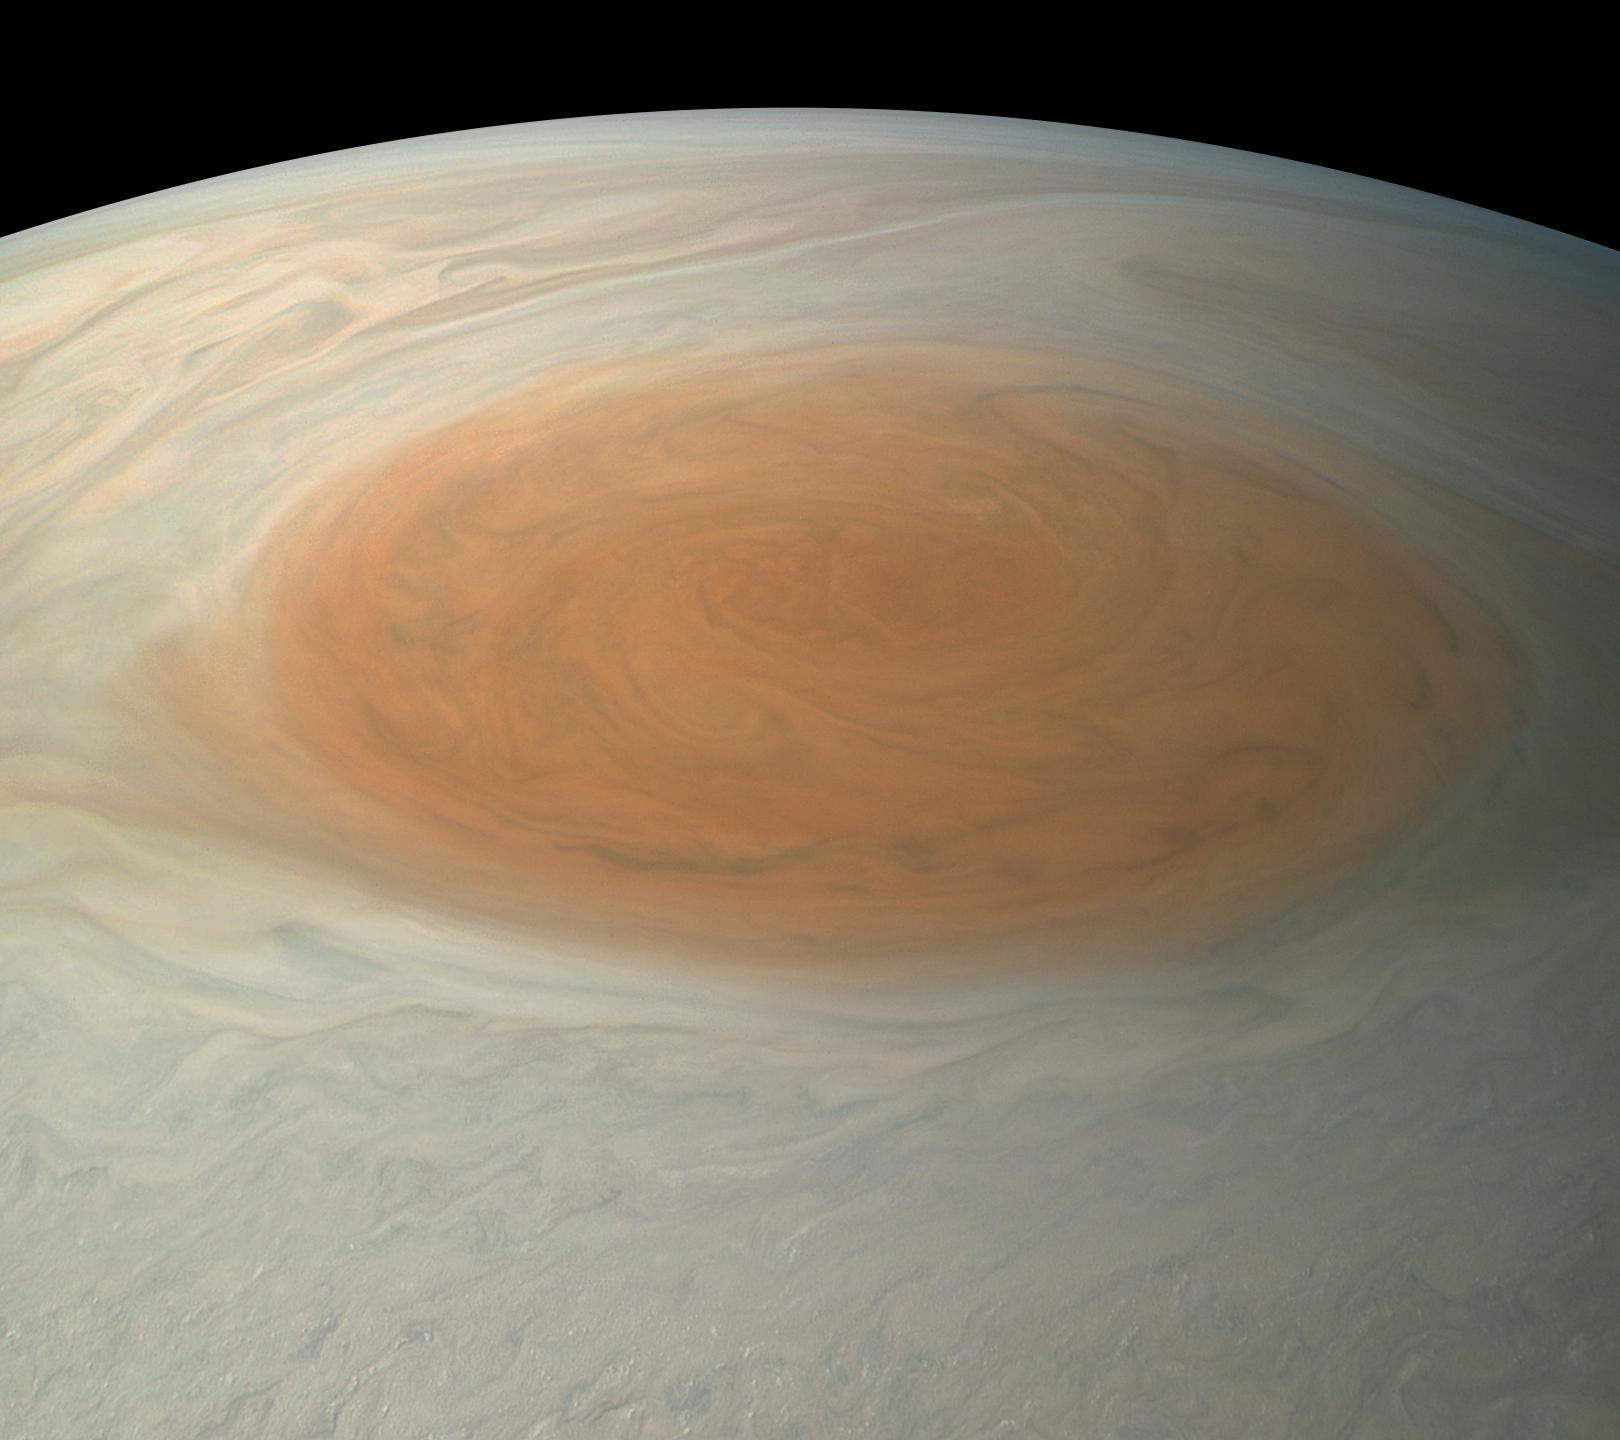
\includegraphics[width=\linewidth,height=0.62\textheight,keepaspectratio]{jupiter_great_red_spot}
    \source{NASA/JPL-Caltech/SwRI/MSSS (Juno)}

    \column{\recaptextcolwide}
    \footnotesize
    \begin{itemize}\setlength\itemsep{2pt}
      \item Anticyclonic vortex larger than Earth; continuous records since $\sim$1830
      \item Peripheral winds reach $\sim$120~m\,s$^{-1}$ between opposing zonal jets
      \item Sustained by merging with smaller vortices and deep $\mathrm{H_2O}$ latent heat release
      \item Slowly shrinking in longitudinal extent over the past century
    \end{itemize}
  \end{columns}
\end{frame}

\begin{frame}
  \centering
  \makebox[\linewidth][c]{\includegraphics[width=0.95\paperwidth, height=0.70\paperheight, keepaspectratio]{juno_polar_cyclones}}\\
  {\footnotesize Polar cyclone cluster at Jupiter's north pole from Juno JIRAM. A central cyclone is encircled by eight circumpolar cyclones in a stable octagonal pattern, demonstrating coherent polygonal vortex dynamics in giant planet atmospheres. Credit: NASA/JPL-Caltech/SwRI/ASI/INAF/JIRAM.}
\end{frame}

% ── Saturn hexagon ──────────────────────────────────────────
\begin{frame}{Saturn: the hexagonal jet stream}
  \begin{columns}[c]
    \column{\recapfigcolnarrow}
    \centering
    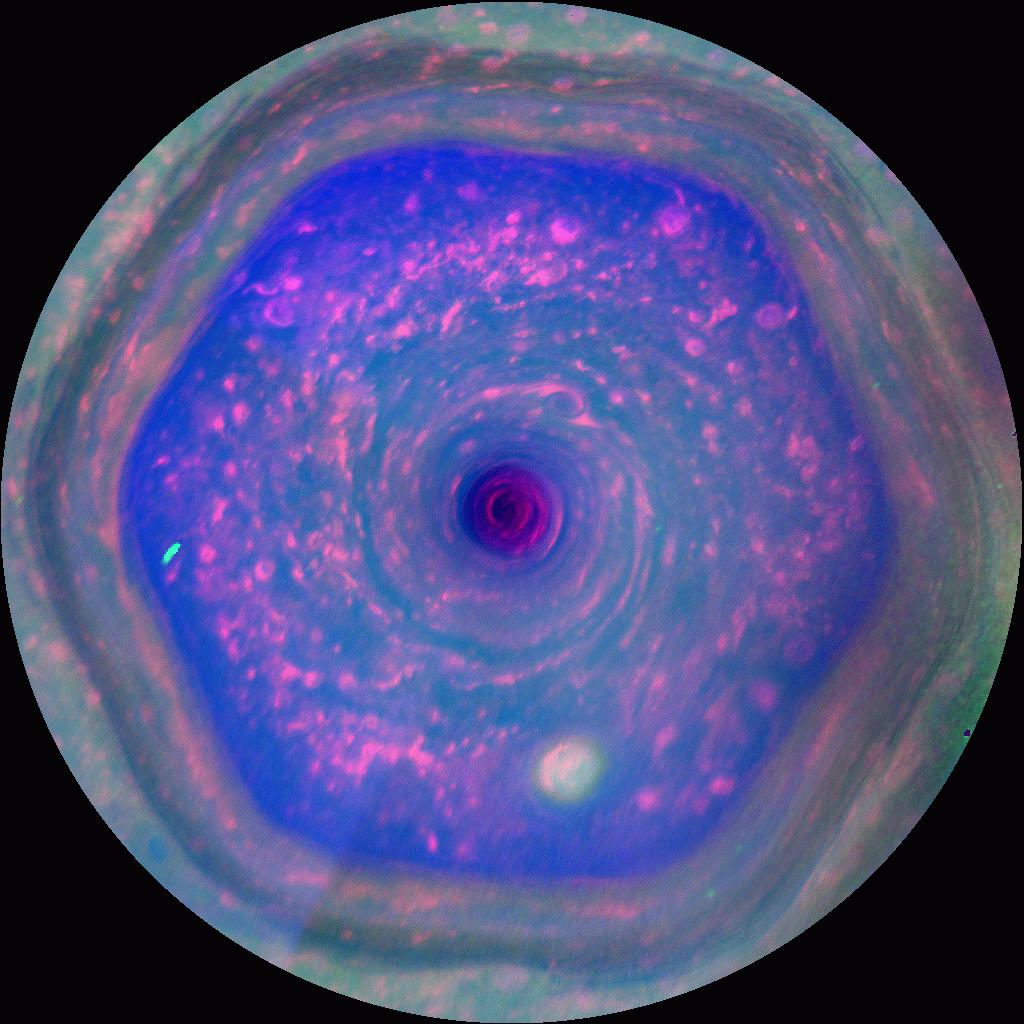
\includegraphics[width=\linewidth,height=0.62\textheight,keepaspectratio]{saturn_hexagon}
    \source{NASA/JPL-Caltech/SSI (Cassini, 2013)}

    \column{\recaptextcolwide}
    \footnotesize
    \begin{itemize}\setlength\itemsep{2pt}
      \item Persistent hexagonal pattern at $\sim$78\textdegree{}N, diameter $\sim$30{,}000~km
      \item Imaged by Voyager (1980--81) and Cassini
      \item Stationary Rossby wave with azimuthal wavenumber $m = 6$ resonant with the zonal jet
      \item Saturn also erupts episodic Great White Storms every $\sim$30~years (last in 2010)
    \end{itemize}
  \end{columns}
\end{frame}

% ── Neptune weather ────────────────────────────────
\begin{frame}
  \centering
  \makebox[\linewidth][c]{\includegraphics[width=0.95\paperwidth, height=0.72\paperheight, keepaspectratio]{neptune_great_dark_spot}}\\
  {\footnotesize Neptune's Great Dark Spot, Voyager 2 (1989). Neptune radiates $\sim$2.6$\times$ more energy than it receives from the Sun, with internal heat driving $\sim$400~m\,s$^{-1}$ winds despite negligible solar heating. Credit: NASA/JPL-Caltech.}
\end{frame}


% ════════════════════════════════════════════════════════════
\sectionimage{snowball_earth}{Snowball Earth, artist's impression. Credit: Oleg Kuznetsov, CC BY-SA 4.0}
\section{Climate evolution \& the faint young Sun}
% ════════════════════════════════════════════════════════════

% ── Faint young Sun curve hero ──────────────────────────────
\begin{frame}
  \centering
  \makebox[\linewidth][c]{\includegraphics[width=0.95\paperwidth, height=0.72\paperheight, keepaspectratio]{feulner2012_solar_luminosity}}\\
  {\footnotesize Solar luminosity across geologic time follows $L(t)/\Lsun \approx [1 + \frac{2}{5}(1 - t/t_\odot)]^{-1}$; at $t = 0$, the Sun was $\sim$30\% fainter ($0.71\,\Lsun$) than today. Reproduced from Feulner (2012).}
\end{frame}

% ── Faint young Sun paradox and solutions ──────────
\begin{frame}{The faint young Sun paradox and solutions}
  A 30\% fainter early Sun implies $T_{\mathrm{eff}} \approx 234$~K, yet geological records require liquid water for $>$4~Gyr.
  \vskip6pt
  \begin{itemize}\setlength\itemsep{3pt}
    \item \textbf{Geological evidence:} zircons (4.4~Ga), pillow basalts (3.8~Ga), and stromatolites (3.5~Ga) prove ancient oceans
    \item \textbf{Paradox:} with today's atmosphere, early Earth would have been globally frozen
    \item \textbf{Solutions:} stronger greenhouse from elevated $\mathrm{CO_2}$ and biogenic $\mathrm{CH_4}$, plus lower continental albedo
  \end{itemize}
\end{frame}

\begin{frame}
  \centering
  \makebox[\linewidth][c]{\includegraphics[width=0.95\paperwidth, height=0.60\paperheight, keepaspectratio]{faint_young_sun}}\\
  {\footnotesize (a) With the solar luminosity at 0.70 of today's value 4.5 Gyr ago, $T_\mathrm{eff} = 255\,(L/L_\odot)^{1/4}$ K starts at 234 K, and even with today's 33 K of greenhouse warming the surface stays below freezing until about 3.2 Ga in this linear approximation; zircons (4.4 Ga), pillow basalts and sedimentary rocks (3.8 Ga) and stromatolites (3.5 Ga) record liquid water instead. (b) The proposed warming contributions: CO$_2$ at 10 to 1000 times present, biogenic CH$_4$, N$_2$ at 2 to 3 times present, and a lower albedo. Course figure.}
\end{frame}

% ── Mars climate puzzle ────────────────────────────
\begin{frame}
  \centering
  \makebox[\linewidth][c]{
\includegraphics[width=0.95\paperwidth, height=0.72\paperheight, keepaspectratio]{mars_valley_networks}}\\
  {\footnotesize Noachian valley networks, Mars Express HRSC. Fluvial networks require warm, wet conditions on early Mars ($>$3.7~Ga), an open paradox under the faint young Sun since pure $\mathrm{CO_2}$ condenses into high-albedo clouds. Credit: ESA/DLR/FU Berlin, CC BY-SA 3.0 IGO.}
\end{frame}

\begin{frame}
  \centering
  \makebox[\linewidth][c]{\includegraphics[width=0.95\paperwidth, height=0.70\paperheight, keepaspectratio]{milankovitch_cycles}}\\
  {\footnotesize Milankovitch cycles over 800~kyr: obliquity, eccentricity, and precession modulate high-latitude summer insolation, pacing glacial cycles observed in ice-core and sediment records, though the 100~kyr rhythm requires non-linear climate feedbacks. Credit: Wikimedia Commons, CC BY-SA.}
\end{frame}

% ── Climate feedbacks and ice-albedo ───────────────
\begin{frame}{Climate feedbacks and the ice-albedo instability}
  Atmospheric feedbacks determine whether a planetary climate remains stable or runs away.
  \vskip6pt
  \begin{itemize}\setlength\itemsep{3pt}
    \item \textbf{Water vapour feedback:} warming increases vapour, doubling $\mathrm{CO_2}$ warming (runaway on Venus)
    \item \textbf{Cloud feedback:} competing solar reflection (cooling) and infrared trapping (warming)
    \item \textbf{Ice-albedo feedback:} cooling expands reflective ice; past $\sim$30\textdegree{} latitude, runaway cooling triggers a snowball state
  \end{itemize}
\end{frame}

% ── Snowball bistability hero ───────────────────────────────
\begin{frame}
  \centering
  \makebox[\linewidth][c]{\includegraphics[width=0.95\paperwidth, height=0.72\paperheight, keepaspectratio]{snowball_bistability}}\\
  {\footnotesize Energy-balance bistability of the ice-albedo feedback. Stable crossings at 250~K and 287~K bracket an unstable threshold at 267~K, separating warm and snowball branches. Course figure.}
\end{frame}

% ── Snowball Earth ──────────────────────────────────────────
\begin{frame}{Snowball Earth}
  \begin{columns}[c]
    \column{\recapfigcolnarrow}
    \centering
    \includegraphics[width=\linewidth,height=0.62\textheight,keepaspectratio]{snowball_earth}
    \source{Oleg Kuznetsov, CC BY-SA 4.0}

    \column{\recaptextcolwide}
    \footnotesize
    \begin{itemize}\setlength\itemsep{2pt}
      \item Two global glaciations in the Neoproterozoic ($\sim$717 and 635~Ma) with tropical glacial deposits
      \item Surface temperatures dropped below $-50$\textdegree C
      \item Global ice cover shut down silicate weathering sinks
      \item Volcanic $\mathrm{CO_2}$ accumulated unchecked over $\sim$10--100~Myr until greenhouse warming melted the ice
    \end{itemize}
    \vskip2pt
    \sourcenote{Hoffman et al.\ (2017)}
  \end{columns}
\end{frame}


% ════════════════════════════════════════════════════════════
\sectionimage{carbonate_silicate_cycle}{Carbonate-silicate cycle. Credit: Wikimedia, CC BY-SA 4.0}
\section{The carbonate-silicate cycle}
% ════════════════════════════════════════════════════════════

% ── Urey reaction ───────────────────────────────────────────
\begin{frame}{The Urey reaction}
  Silicate weathering draws atmospheric $\mathrm{CO_2}$ dissolved in rainwater into mineral carbonates:
  \vskip6pt
  \keyresult{$$\mathrm{CaSiO_3} + \mathrm{CO_2} + \mathrm{H_2O} \longrightarrow \mathrm{CaCO_3} + \mathrm{SiO_2} + \mathrm{H_2O}$$}
  \vskip6pt
  \begin{itemize}\setlength\itemsep{2pt}
    \item Atmospheric $\mathrm{CO_2}$ dissolves in rain forming carbonic acid ($\mathrm{H_2CO_3}$)
    \item Acid weathers surface silicates, washing $\mathrm{Ca}^{2+}$ and $\mathrm{HCO_3^-}$ to the oceans
    \item Marine organisms and abiotic processes precipitate carbonate sediments ($\mathrm{CaCO_3}$)
    \item Net effect: moves carbon from the atmosphere-ocean system into the crust, until subduction and volcanism return it
  \end{itemize}
\end{frame}

\begin{frame}
  \centering
  \makebox[\linewidth][c]{\includegraphics[width=0.95\paperwidth, height=0.62\paperheight, keepaspectratio]{urey_reaction_pathway}}\\
  {\footnotesize The Urey reaction pathway: CO$_2$ dissolves in rainwater as a weak carbonic acid, weathers CaSiO$_3$, rivers carry Ca$^{2+}$, HCO$_3^-$ and SiO$_2$ to the ocean, and CaCO$_3$ precipitates and is deposited as sedimentary rock. Net effect: CO$_2$ drawn out of the atmosphere into carbonate rock, the long-term carbon sink. Course schematic.}
\end{frame}

\begin{frame}
  \centering
  \makebox[\linewidth][c]{\includegraphics[width=0.95\paperwidth, height=0.72\paperheight, keepaspectratio]{foley2024_carbonate_silicate}}\\
  {\footnotesize Carbonate-silicate cycle on the modern Earth. Atmospheric $\mathrm{CO_2}$ dissolves in rainwater, weathers surface silicates into oceanic carbonates, and plate-tectonic subduction returns metamorphic $\mathrm{CO_2}$ to the atmosphere via arc and plume volcanism. Credit: Foley (2024).}
\end{frame}

% ── Volcanic source ─────────────────────────────────────────
\begin{frame}{Volcanic outgassing: the carbon source}
  \begin{columns}[c]
    \column{\recapfigcolnarrow}
    \centering
    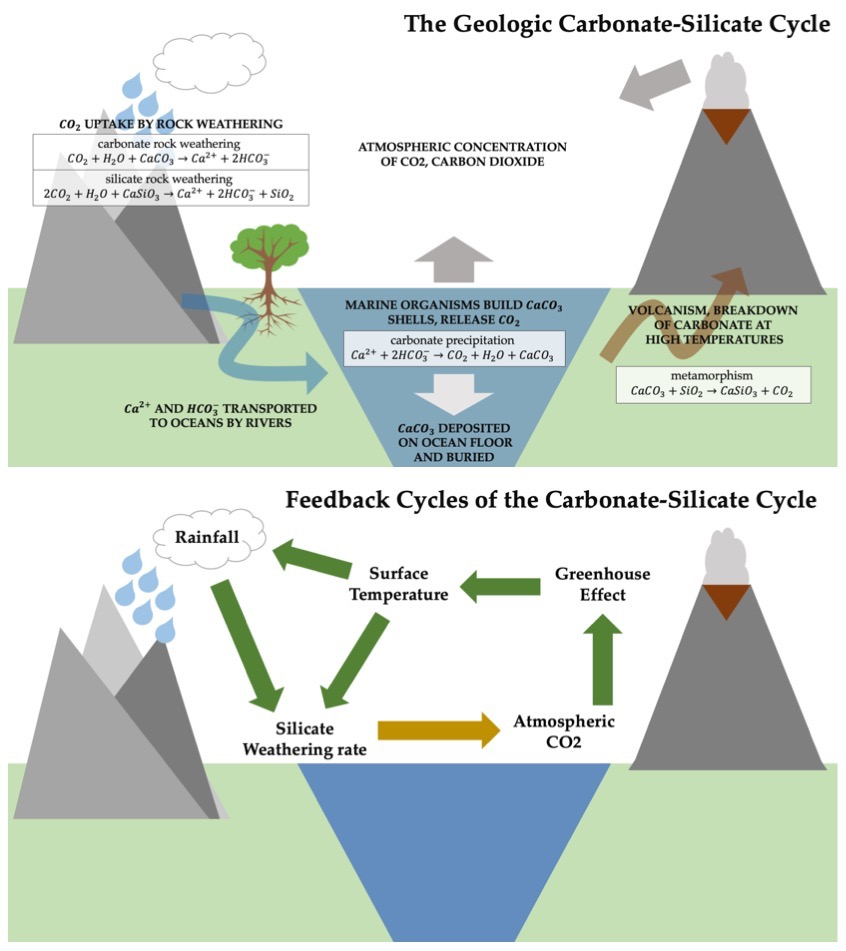
\includegraphics[width=\linewidth,height=0.62\textheight,keepaspectratio]{carbonate_silicate_cycle}
    \source{Wikimedia, CC BY-SA 4.0}

    \column{\recaptextcolwide}
    \footnotesize
    \begin{itemize}\setlength\itemsep{2pt}
      \item Plate tectonics subducts carbonate-rich seafloor into the mantle
      \item High $T$ and $P$ decompose carbonates, releasing metamorphic $\mathrm{CO_2}$
      \item \textbf{Volcanic outgassing} returns $\mathrm{CO_2}$ to the atmosphere
      \item Long-term steady state balances weathering sinks against volcanic sources
    \end{itemize}
  \end{columns}
\end{frame}

% ── Negative feedback thermostat ───────────────────────────
\begin{frame}{The negative feedback thermostat}
  Silicate weathering provides temperature-dependent negative feedback:
  \vskip6pt
  \begin{itemize}\setlength\itemsep{3pt}
    \item \textbf{Warming:} higher rainfall and reaction rates accelerate weathering, drawing down $\mathrm{CO_2}$ and cooling the planet
    \item \textbf{Cooling:} reduced weathering allows volcanic $\mathrm{CO_2}$ to accumulate, strengthening the greenhouse
  \end{itemize}
  \vskip6pt
  \keyresult{Operates on $\sim$0.5~Myr timescales, maintaining liquid water for $>$4~Gyr.}
\end{frame}

% ── Quantifying weathering feedback ────────────────────────
\begin{frame}{Quantifying the weathering feedback}
  Silicate weathering rates increase exponentially with temperature to stabilise climate:
  $$W(T) = W_0 \exp\!\left(\frac{T - T_0}{T_e}\right)$$
  \vskip4pt
  \begin{itemize}\setlength\itemsep{2pt}
    \item With $T_e \approx 10$~K, doubling weathering requires $\sim$7~K warming
    \item Climate perturbations damp on a $\sim$0.5~Myr timescale
    \item Feedback requires liquid water and active volcanism to operate
  \end{itemize}
  \vskip2pt
  \sourcenote{Walker et al.\ (1981); Pierrehumbert (2010)}
\end{frame}

% ── Venus and Mars: failed thermostats ──────────────────────
\begin{frame}{Venus \& Mars: failed thermostats}
  \footnotesize
  The thermostat requires liquid water and volcanism:
  \vskip4pt
  \begin{columns}[T]
    \column{0.48\textwidth}
    \textbf{Venus (lost sink):}
    \begin{itemize}\setlength\itemsep{1pt}
      \item Runaway greenhouse boiled oceans
      \item No water $\rightarrow$ no weathering sink
      \item Volcanic $\mathrm{CO_2}$ reached 92~bar
    \end{itemize}

    \column{0.48\textwidth}
    \textbf{Mars (lost source):}
    \begin{itemize}\setlength\itemsep{1pt}
      \item Volcanism ceased $\sim$3~Ga
      \item No volcanic return path
      \item Weathering drawdown and escape left $\sim$6~mbar
    \end{itemize}
  \end{columns}
  \vskip4pt
  \keyresult{Habitability requires active geological cycling, not sunlight alone.}
\end{frame}

\begin{frame}
  \centering
  \makebox[\linewidth][c]{\includegraphics[width=0.95\paperwidth, height=0.64\paperheight, keepaspectratio]{thermostat_failure}}\\
  {\footnotesize The thermostat needs both ingredients: Earth has liquid water and active volcanism and regulates CO$_2$ over Gyr; Venus lost its water, so weathering stopped and volcanic CO$_2$ accumulated to 92 bar; Mars lost its volcanism after about 3 Ga, so weathering and escape drew CO$_2$ down to 6 mbar; with neither there is no cycle. Course schematic.}
\end{frame}


% ════════════════════════════════════════════════════════════
\sectionimage{mars_dust_storm}{Mars global dust storm (2018). Credit: NASA/JPL-Caltech/MSSS}
\section{Recent advances \& outlook}
% ════════════════════════════════════════════════════════════

% ── Venus phosphine hero ────────────────────────────────────
\begin{frame}
  \centering
  \makebox[\linewidth][c]{\includegraphics[width=0.95\paperwidth, height=0.72\paperheight, keepaspectratio]{lincowski2021_phosphine_so2}}\\
  {\footnotesize The reported 267~GHz Venus phosphine feature is fit by mesospheric $\mathrm{SO_2}$, a controversy that NASA's DAVINCI descent probe will test in situ. Lincowski et al.\ (2021).}
\end{frame}

% ── Summary ────────────────────────────────────────────────
\begin{frame}{Summary}
  \begin{enumerate}\setlength\itemsep{2pt}
    \item Clausius-Clapeyron equation predicts saturation vapour pressure and cloud bases
    \item Planetary rotation sets circulation cells, from single Hadley loops to banded jets
    \item Geostrophic balance and thermal wind govern large-scale winds and storms
    \item Faint young Sun paradox is resolved by greenhouse warming and lower albedo
    \item Carbonate-silicate weathering provides a $\sim$0.5~Myr climate thermostat
  \end{enumerate}
  \vskip6pt
  \textbf{Next: Lecture 7}
\end{frame}

% ── Final slide ─────────────────────────────────────────────
\begin{frame}[plain,noframenumbering]
  \begin{tikzpicture}[remember picture, overlay]
    \ipscontain{title_background}
    \fill[ipsPrimary, opacity=0.70] (current page.north west) rectangle (current page.south east);
  \end{tikzpicture}
  \vfill
  \begin{center}
    {\color{white}\Large\bfseries Questions?}
    \vskip20pt
    {\color{white!85}\large Next: Lecture 7, Planetary surfaces: geology, geomorphology \& geophysics}\\[4pt]
    {\color{white!85}\small Mon 28 Sep, 15:00--17:00, room 5419.0161 (Collegezaal)}\\[12pt]
    {\color{white!85}\small Next tutorial: Fri 25 Sep, 13:00--15:00, room 5419.0161 (Collegezaal)}\\[20pt]
    {\color{white!70}\small \texttt{https://ips.formingworlds.space}}
  \end{center}
  \vfill
\end{frame}

\end{document}
